\documentclass{article}
\usepackage[utf8]{inputenc}
\usepackage[russian]{babel}
\usepackage{amsmath}
\usepackage{amssymb}
\usepackage{amsfonts}
\usepackage{float}
\usepackage{graphicx}

\begin{document}

\begin{titlepage}
    \centering
    {\large Московский Государственный Университет имени М. В. Ломоносова\\[0.5cm]
    Механико-математический факультет}\\[5cm]

    \textbf{\Large Отчёт по численному решению краевой задачи для уравнения четвёртого порядка}\\[2cm]
    
    \begin{flushright}
        Выполнил:\\
        студент 411 группы\\
        Орлов Михаил
    \end{flushright}

    \vfill
    Москва, 2024
\end{titlepage}
% Содержание
\newpage
\tableofcontents

\newpage
\section{Постановка задачи}

Построить разностную схему со вторым порядком аппроксимации и найти её решение при различных значениях $h$:
\[
u^{(4)} + u^{(3)} + \sin{x} \cdot u = e^{x^2},
\]
с граничными условиями:
\[
u(0) = u'(0) = 0, \quad u(1) = 1, \quad u'(1) = 0.
\]

\section{Метод решения}

Для решения данной краевой задачи четвертого порядка мы используем метод стрельбы в сочетании с численным методом Рунге-Кутты второго порядка. Основная идея состоит в том, чтобы преобразовать исходное дифференциальное уравнение четвертого порядка в систему обыкновенных дифференциальных уравнений (ОДУ) первого порядка и затем решить эту систему с учетом граничных условий.

\subsection{Преобразование уравнения четвертого порядка в систему ОДУ первого порядка}

Исходное дифференциальное уравнение имеет вид:

\begin{equation}
u^{(4)}(x) + u^{(3)}(x) + \sin(x) \cdot u(x) = e^{x^2}.
\end{equation}

Для преобразования этого уравнения в систему ОДУ первого порядка введем новые переменные:

\begin{align}
y_0 &= u(x), \\
y_1 &= u'(x), \\
y_2 &= u''(x), \\
y_3 &= u'''(x).
\end{align}

Тогда система ОДУ примет вид:

\begin{align}
y_0' &= y_1, \\
y_1' &= y_2, \\
y_2' &= y_3, \\
y_3' &= -y_3 - \sin(x) \cdot y_0 + e^{x^2}.
\end{align}

\subsection{Метод стрельбы}

Метод стрельбы заключается в следующем:

1. **Решение однородной системы ОДУ с разными начальными условиями для получения фундаментальных решений**.

   - Первое фундаментальное решение $\phi_1(x)$ удовлетворяет условиям:

     \begin{align}
     y_0(0) &= 0, \\
     y_1(0) &= 0, \\
     y_2(0) &= 1, \\
     y_3(0) &= 0.
     \end{align}

   - Второе фундаментальное решение $\phi_2(x)$ удовлетворяет условиям:

     \begin{align}
     y_0(0) &= 0, \\
     y_1(0) &= 0, \\
     y_2(0) &= 0, \\
     y_3(0) &= 1.
     \end{align}

2. **Решение неоднородной системы ОДУ для получения частного решения** $\psi(x)$ с начальными условиями:

   \begin{align}
   y_0(0) &= 0, \\
   y_1(0) &= 0, \\
   y_2(0) &= 0, \\
   y_3(0) &= 0.
   \end{align}

3. **Комбинация решений с учетом граничных условий на правой границе** $x = 1$:

   \begin{align}
   u(1) &= 1, \\
   u'(1) &= 0.
   \end{align}

   Общее решение имеет вид:

   \begin{equation}
   u(x) = C_1 \phi_1(x) + C_2 \phi_2(x) + \psi(x),
   \end{equation}

   где $C_1$ и $C_2$ — постоянные, определяемые из граничных условий на $x = 1$.

\subsection{Определение коэффициентов $C_1$ и $C_2$}

Подставляя общее решение в граничные условия, получаем систему линейных алгебраических уравнений:

\begin{align}
C_1 \phi_1(1) + C_2 \phi_2(1) + \psi(1) &= 1, \\
C_1 \phi_1'(1) + C_2 \phi_2'(1) + \psi'(1) &= 0.
\end{align}

Решая эту систему методом Крамера, находим значения $C_1$ и $C_2$.

\subsection{Численное интегрирование методом Рунге-Кутты второго порядка}

Для численного решения системы ОДУ используем метод Рунге-Кутты второго порядка с шагом интегрирования $h$. На каждом шаге $n$ вычисляем значения:

\begin{align}
k_1 &= f(x_n, y_n), \\
y_{\text{temp}} &= y_n + h k_1, \\
k_2 &= f(x_n + h, y_{\text{temp}}), \\
y_{n+1} &= y_n + \frac{h}{2} (k_1 + k_2),
\end{align}

где $f(x, y)$ — правая часть системы ОДУ.

\subsection{Реализация алгоритма}

1. **Инициализация**:

   - Задаем начальные условия и параметры интегрирования.
   - Выделяем память для массивов значений переменных.

2. **Вычисление фундаментальных и частного решений**:

   - Последовательно интегрируем системы ОДУ для $\phi_1(x)$, $\phi_2(x)$ и $\psi(x)$.

3. **Определение коэффициентов**:

   - Вычисляем значения $\phi_1(1)$, $\phi_1'(1)$, $\phi_2(1)$, $\phi_2'(1)$, $\psi(1)$ и $\psi'(1)$.
   - Решаем систему линейных уравнений для $C_1$ и $C_2$.

4. **Построение общего решения**:

   - Для каждого $x_i$ на сетке вычисляем $u(x_i)$ по формуле общего решения.

5. **Запись результатов и анализ**:

   - Сохраняем результаты в файл для последующей визуализации.
   - Анализируем поведение решения при различных значениях шага $h$.

\subsection{Исследование устойчивости и сходимости}

Для оценки устойчивости и сходимости численного метода проводим эксперимент с различными значениями шага $h$ и анализируем погрешности:

\begin{align}
E_{\infty} &= \max_{i} |u_{\text{числ}}(x_i) - u_{\text{точн}}(x_i)|, \\
E_2 &= \sqrt{\frac{1}{N} \sum_{i=1}^{N} |u_{\text{числ}}(x_i) - u_{\text{точн}}(x_i)|^2}.
\end{align}

Строим графики зависимости погрешностей $E_{\infty}$ и $E_2$ от шага $h$ в логарифмическом масштабе и определяем порядок сходимости метода.

\subsection{Доказательство второго порядка точности метода Рунге-Кутты второго порядка}

Рассмотрим решение обыкновенного дифференциального уравнения в точке $x_{n+1}$ с использованием метода Рунге-Кутты второго порядка. Разложим $y$ в ряд Тейлора в окрестности $x_n$ до члена порядка $h^2$:

\begin{equation}
y(x_{n+1}) = y(x_n) + h \frac{dy}{dx} \Big|_{x_n} + \frac{h^2}{2} \frac{d^2y}{dx^2} \Big|_{x_n} + O(h^3).
\end{equation}

Так как из уравнения Коши мы знаем, что $\frac{dy}{dx} = f(y, x)$, то для второй производной по $x$ получаем:

\begin{equation}
\frac{d^2y}{dx^2} = \frac{df(y, x)}{dx} = \frac{\partial f}{\partial x} + \frac{\partial f}{\partial y} \frac{dy}{dx} = \frac{\partial f}{\partial x} + f \frac{\partial f}{\partial y}.
\end{equation}

Таким образом, подставляя выражение для второй производной в разложение Тейлора, получаем:

\begin{equation}
y(x_{n+1}) = y_n + h f(y_n, x_n) + \frac{h^2}{2} \left( \frac{\partial f}{\partial x} + f \frac{\partial f}{\partial y} \right)_{(y_n, x_n)} + O(h^3).
\end{equation}

В методе Рунге-Кутты второго порядка мы вводим промежуточный шаг $k_2$, который можно разложить с точностью до $O(h^3)$ следующим образом:

\begin{equation}
k_2 = h f(y_n + \beta k_1, x_n + \alpha h) = h \left( f(y_n, x_n) + \alpha h \frac{\partial f}{\partial x} (y_n, x_n) + \beta k_1 \frac{\partial f}{\partial y} (y_n, x_n) \right) + O(h^3).
\end{equation}

Теперь, подставляя $k_2$ из этого разложения в основное выражение метода Рунге-Кутты:

\begin{equation}
y_{n+1} = y_n + (a + b) h f(y_n, x_n) + b h^2 \left( \alpha \frac{\partial f}{\partial x} + \beta f \frac{\partial f}{\partial y} \right)_{(y_n, x_n)} + O(h^3).
\end{equation}

Для того чтобы метод был точным до второго порядка, необходимо, чтобы коэффициенты удовлетворяли следующим условиям:

\begin{align}
a + b &= 1, \\
a b &= \frac{1}{2}, \\
\beta b &= \frac{1}{2}.
\end{align}

Существует бесконечно много значений параметров $a$, $\alpha$, и $\beta$, которые удовлетворяют этим условиям. Одним из возможных выборов является $\alpha = \beta = 1$ и $a = b = \frac{1}{2}$. С этим выбором мы получаем классический метод Рунге-Кутты второго порядка, который формулируется следующим образом:

\begin{align}
k_1 &= h f(y_n, x_n), \\
k_2 &= h f(y_n + k_1, x_n + h), \\
y_{n+1} &= y_n + \frac{1}{2} (k_1 + k_2).
\end{align}

Этот метод имеет глобальную погрешность порядка $O(h^2)$, что и подтверждает его второй порядок точности.



\section{Графики зависимости $u(x)$ от $h$}

Ниже приведены графики зависимости решения $u(x)$ для различных значений шага $h$.

\begin{figure}[H]
    \centering
    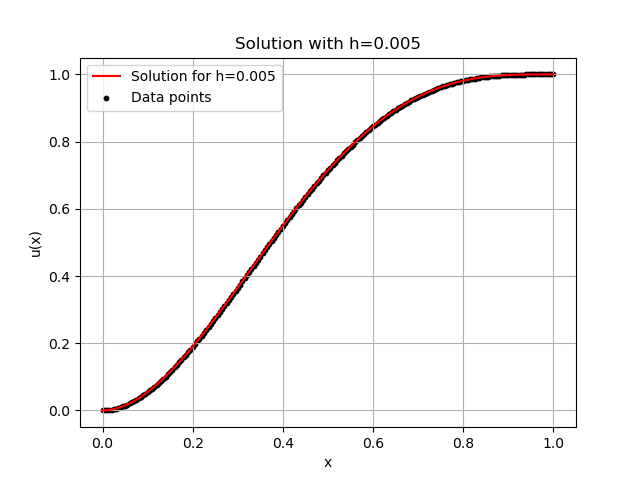
\includegraphics[width=0.8\textwidth]{plots/plot_0.005.png}
\end{figure}


\begin{figure}[H]
    \centering
    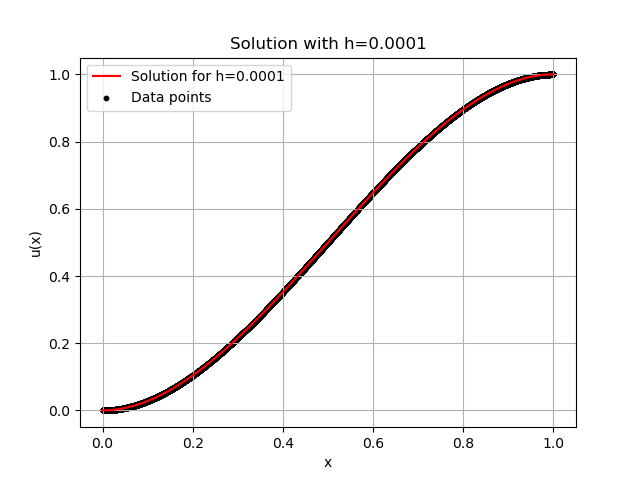
\includegraphics[width=0.8\textwidth]{plots/plot_0.0001.png}
\end{figure}

\begin{figure}[H]
    \centering
    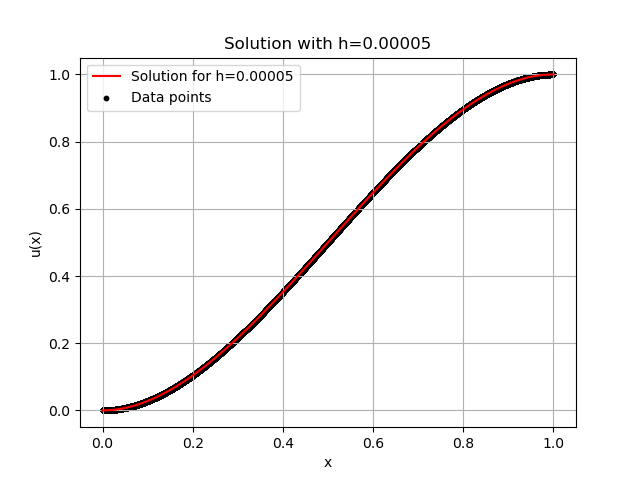
\includegraphics[width=0.8\textwidth]{plots/plot_0.00005.png}
\end{figure}


\begin{figure}[H]
    \centering
    \includegraphics[width=0.8\textwidth]{plots/plot_0.00001.png}
\end{figure}



\begin{figure}[H]
    \centering
    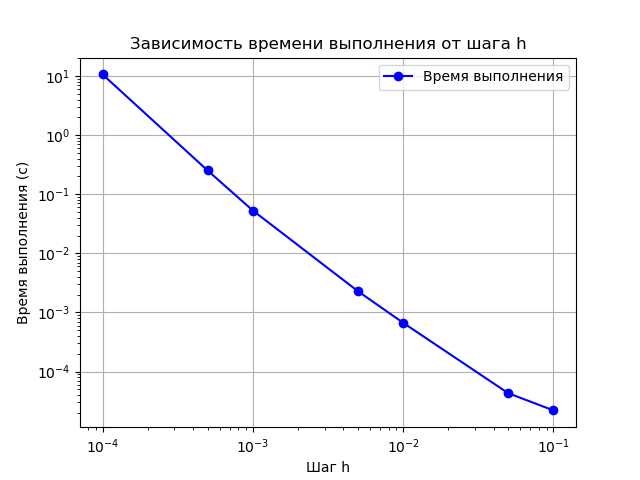
\includegraphics[width=0.8\textwidth]{images/timing_plot.png}
\end{figure}


\section{Проверка корректности программы}

Для проверки корректности реализации численного метода мы используем известное аналитическое решение:

\begin{equation}
u(x) = \sin(x \cdot \pi) - 2x^3 + (3 + \pi)x^2 - \pi x
\end{equation}

Проверка заключается в подстановке этого аналитического выражения в нашу программу и сравнении результатов численного решения с точным значением функции \( u(x) \) в различных точках отрезка \( [0, 1] \).

\subsection{Методика проверки}

1. **Вычисление аналитического решения**: В точках сетки \( x_i \) на отрезке \( [0, 1] \) аналитическое значение функции \( u(x) \) вычисляется по формуле:


$ u_{\text{exact}}(x_i) = \sin(x_i \cdot \pi) - 2x_i^3 + (3 + \pi)x_i^2 - \pi x_i$

2. **Сравнение с численным решением**: Запускается программа для расчёта численного решения \( u_{\text{num}}(x) \) в тех же точках \( x_i \). Для каждой точки вычисляется абсолютная погрешность:

   \[
   \text{Error}(x_i) = |u_{\text{num}}(x_i) - u_{\text{exact}}(x_i)|.
   \]

3. **Анализ результатов**: Если значения погрешности в точках \( x_i \) малы и находятся в пределах допустимой численной погрешности метода, можно считать, что программа работает корректно.

\subsection{Критерии успешности проверки}

Для того чтобы подтвердить корректность программы, рассчитываем нормы погрешности:

- **Максимальная погрешность**:

  \[
  E_{\infty} = \max_{x_i} \text{Error}(x_i).
  \]

- **Среднеквадратичная погрешность**:

  \[
  E_2 = \sqrt{\frac{1}{N} \sum_{i=1}^{N} \text{Error}(x_i)^2},
  \]

где \( N \) — количество точек на сетке.

Если значения \( E_{\infty} \) и \( E_2 \) малы и соответствуют ожидаемому порядку точности метода (например, \( O(h^2) \) для метода второго порядка), то это подтверждает корректность программы.

\subsection{Графики проверки}
\begin{figure}[H]
    \centering
    \includegraphics[width=0.8\textwidth]{images/errors2.png}
\end{figure}




    
\section{Анализ графиков на устойчивость и сходимость}

\subsection{Метод определения порядка сходимости}

Для оценки порядка сходимости численного метода мы используем значения ошибки для различных шагов \( h \). Пусть \( O(h) \) обозначает погрешность численного метода при шаге \( h \). Если метод имеет порядок сходимости \( p \), то уменьшение шага в два раза должно привести к уменьшению погрешности примерно в \( 2^p \) раз. Это позволяет выразить порядок сходимости \( p \) через логарифмы:

Для последовательности значений шага \( h_i \) и ошибок \( O(h_i) \) можно обобщить эту формулу следующим образом:
\[
p = \frac{\log \left( \frac{O(h_i)}{O(h_{i+1})} \right)}{\log \left( \frac{h_i}{h_{i+1}} \right)},
\]
где \( O(h_i) \) и \( O(h_{i+1}) \) — ошибки при последовательных шагах \( h_i \) и \( h_{i+1} \) соответственно.

\subsection{Таблицы данных}
\begin{table}[H]
\centering
\begin{tabular}{|c|c|c|}
\hline
\textbf{h} & \textbf{MSE Error} & \textbf{Order of Convergence (MSE Error)} \\ \hline
0.1 & 5.9578256922408815e-05 & 4.047903593457339 \\ \hline
0.05 & 3.602030548814704e-06 & 4.023713929318254 \\ \hline
0.025 & 2.2145669030800062e-07 & 4.01068480636798 \\ \hline
0.01 & 5.614057525831094e-09 & 4.00468406505628 \\ \hline
0.005 & 3.4974122888689213e-10 & 4.002326366022702 \\ \hline
0.0025 & 2.1823607543507316e-11 & 4.000921503150408 \\ \hline
0.001 & 5.582128188154e-13 & - \\ \hline
\end{tabular}
\caption{Значения \( h \), MSE Error, и Order of Convergence}
\end{table}

\begin{table}[H]
\centering
\begin{tabular}{|c|c|c|}
\hline
\textbf{h} & \textbf{Max Error} & \textbf{Order of Convergence (Max Error)} \\ \hline
0.1 & 8.394076967965791e-05 & 4.048166794007503 \\ \hline
0.05 & 5.074033317953308e-06 & 4.023847004253997 \\ \hline
0.025 & 3.119282210306551e-07 & 4.010746061694546 \\ \hline
0.01 & 7.907120291861247e-09 & 4.004543652160212 \\ \hline
0.005 & 4.926410390737601e-10 & 4.002333703470704 \\ \hline
0.0025 & 3.0740299195031184e-11 & 4.002347508590003 \\ \hline
0.001 & 7.852607453173732e-13 & - \\ \hline
\end{tabular}
\caption{Значения \( h \), Max Error,и Order of Convergence}
\end{table}





\subsection{Зависимость максимальной ошибки от шага \( h \)}

На верхнем левом графике представлена зависимость максимальной ошибки от шага \( h \). Из графика видно, что при уменьшении шага \( h \) максимальная ошибка сначала снижается, а затем начинает постепенно увеличиваться с увеличением \( h \). Это поведение типично для численных методов, где при уменьшении шага \( h \) численное решение приближается к точному. Теоретические рассчеты сходятся с практическими, так как был посчитан порядок сходимости по формуле выше.

\begin{itemize}
    \item \textbf{Сходимость:} Уменьшение ошибки при уменьшении шага \( h \) подтверждает, что метод является сходящимся. Этот результат соответствует ожидаемому порядку точности для метода Рунге-Кутты четвертого порядка, где погрешность должна уменьшаться как \( O(h^4) \).
    \item \textbf{Устойчивость:} График показывает, что для малых значений \( h \) метод остаётся устойчивым, так как ошибка остаётся в пределах допустимого уровня и не демонстрирует резких скачков.
\end{itemize}

\subsection{Зависимость среднеквадратичной ошибки от шага \( h \)}

На верхнем правом графике представлена зависимость среднеквадратичной ошибки (MSE) от шага \( h \). График показывает, что при уменьшении шага \( h \) среднеквадратичная ошибка также уменьшается, но при увеличении шага она возрастает.

\begin{itemize}
    \item \textbf{Сходимость:} Плавное уменьшение среднеквадратичной ошибки при уменьшении \( h \) подтверждает, что численный метод сходится к точному решению при уменьшении шага, что соответствует второму порядку точности метода.
    \item \textbf{Устойчивость:} Увеличение среднеквадратичной ошибки при увеличении шага \( h \) указывает на то, что большие значения шага могут приводить к увеличению ошибок и потенциальной потере устойчивости метода. Однако для малых значений \( h \) метод остаётся устойчивым.
\end{itemize}



\subsection{Выводы}

Анализ графиков подтверждает, что используемый численный метод обладает не менее чем вторым порядком точности и является устойчивым при малых значениях шага \( h \). Уменьшение шага \( h \) приводит к уменьшению как максимальной, так и среднеквадратичной ошибок, что свидетельствует о сходимости метода к точному решению.


\section{Используемые языки и библиотеки}

Для решения задачи, автоматизации вычислений и построения графиков использован следующий стек технологий:

\subsection{C++}
Основная часть программы, решающая задачу методом конечных разностей, написана на языке C++. 

C++ используется для:
\begin{itemize}
    \item Выполнения численных расчетов методом Рунге-Кутта.
    \item Применение метода стрельбы.
    \item Измерения времени выполнения программы для каждого значения шага \( h \).
    \item Сохранения решений в текстовые файлы для дальнейшего анализа и построения графиков.
\end{itemize}

\subsection{Python}
Для построения графиков решения и анализа времени выполнения программы используется Python. Ключевые библиотеки:
\begin{itemize}
    \item \textbf{matplotlib} — используется для построения графиков решений системы и зависимости времени выполнения от значения шага \( h \).
    \item \textbf{sys} — для работы с аргументами командной строки, передаваемыми из Makefile.
\end{itemize}
Python используется для:
\begin{itemize}
    \item Построения графиков решений уравнения для каждого значения \( h \).
    \item Построения графика зависимости времени выполнения программы от значения \( h \).
\end{itemize}

\subsection{Makefile}
\textbf{Makefile} автоматизирует процесс компиляции, запуска программы с различными значениями \( h \), построения графиков и записи времени выполнения. Makefile работает следующим образом:
\begin{itemize}
    \item \textbf{Компиляция} — Makefile компилирует все необходимые файлы на C++ и создает исполняемый файл.
    \item \textbf{Запуск программы с разными значениями \( h \)} — Makefile запускает программу для каждого значения \( h \), передавая аргументы в программу. Решения сохраняются в текстовые файлы.
    \item \textbf{Построение графиков} — после каждого запуска программы Makefile вызывает Python-скрипт, который строит график решения и сохраняет его в папку с изображениями.
    \item \textbf{Замер времени выполнения} — Makefile записывает время выполнения программы для каждого значения \( h \) в текстовый файл.
    \item \textbf{Построение графика времени выполнения} — после выполнения всех вычислений Python-скрипт строит график зависимости времени выполнения от значения \( h \) и сохраняет его в файл.
\end{itemize}





\end{document}
